\documentclass[times, utf8, diplomski]{fer}
\usepackage{booktabs}

\newcommand{\bplus}{B\textsuperscript{+}}
\newcommand{\rstar}{R\textsuperscript{*}}

\usepackage{graphicx}
\graphicspath{ {images/} }
\usepackage{listings}

\begin{document}

% TODO: Navedite broj rada.
\thesisnumber{1290}

% TODO: Navedite naslov rada.
\title{System for tracking vehicle locations in real time}

% TODO: Navedite vaše ime i prezime.
\author{Frane Kurtović}

\maketitle

% Ispis stranice s napomenom o umetanju izvornika rada. Uklonite naredbu \izvornik ako želite izbaciti tu stranicu.
\izvornik

% Dodavanje zahvale ili prazne stranice. Ako ne želite dodati zahvalu, naredbu ostavite radi prazne stranice.
\zahvala{Zahvala}

\tableofcontents















% --------------INTRODUCTION-------------------------------------------------------------------------------------------------
\chapter{Introduction}
Combining the GPS and mobile technologies it is becoming easier than ever to track the geographical location of a large number of vehicles. Sensors on each vehicle send location updates every few seconds and the users of such system should be able to see which vehicles are currently located in certain area. This thesis will focus on building a \emph{backend part} of this vehicle tracking system. The system has to be able to achieve high throughput of updates and searches, and this must not be limited by the performance capabilities of a single machine. This is why the main design aspect is the ability to \emph{scale on multiple machines}.

Before defining an exact version of the problem, it is good to take a look on what are the possible options to choose from. Vehicle location is a multidimensional data point, it can contain up to three dimensions of spatial data and even one dimension of temporal data. Dataset is comprised of many data points and can be either static or live -- in terms of supporting updates of vehicle locations. Of course, data is not worth anything if it can't be queried. Some common queries can be to search for points contained in a given rectangle, or even more general in an arbitrary polygon. Also, a similar query is to find the points contained within certain radius of a given point, but then another question arises -- how is distance defined in this space. A natural assumption is that the points are on planet Earth, but even Earth can be modelled in many ways, as a perfect sphere or as an ellipsoid, each one suitable for a different application in life. If temporal dimension is present then all of these queries can be appended with time interval to return only the points that happened within that time.

% Another possibility is to add information about road positions and then try to match each vehicle to the closest point on the road. This means that a polygon query could be done in 

\section{Motivation}
Spatial and spatio-temporal data sets are growing rapidly. Consider these spatio-temporal data sets: Facebook or Foursquare with their check-ins, or photos on Instagram. These are all live datasets because queries and updates happen concurrently. There are also examples of static data sets such as data collected by Telecom providers -- a data point for each time a user's phone contacted the tower. This dataset is not live and could be used to perform analytics, usually in a MapReduce system, which has much different requirements on the design of the system.

Initial inspiration for the problem is Uber and similar applications. They have a large number of vehicles that update their location every few seconds. Each user's phone shows vehicles that are in a relatively small area of the map which gives a pretty clear picture of what the most relevant queries could be. Note that this is not a spatio-temporal dataset because only the last location of a vehicle is important, although one could easily imagine the version where the history of locations is stored and queried.

\section{Problem definition and constraints}
Let us define the problem more precisely. Each vehicle has a unique vehicle id and location. Location is encoded in a standard geographic coordinate system, as longitude and latitude pairs. Longitude is in [-180, 180] range and latitude [-90, 90].

Updating a location can be referred as \emph{update $(vehicle\_id, longitude, latitude$)}.

The simplest possible query is to find a list of vehicles that are within a given rectangle, and is referred as
$$rectangle\_query (longitude\_min, longitude\_max, latitude\_min, latitude\_max)$$
A point with its longitude and latitude is inside a given rectangle iff $longitude\_min \le longitude \le longitude\_max$ and $latitude\_min \le latitude \le latitude\_max$.

Another interesting query is to search for points within certain distance of a given point.  Let's refer to this query as
$$radius\_query (longitude, latitude, radius)$$

Notice that the rectangle query was defined in a general way, it could be applied to any two dimensional data set, but this query needs a definition of distance between two points. We will use the simplest Earth model, a perfect sphere with quadratic mean radius of 6372 km. This choice is acceptable because distances should be fairly small and precise geometrical calculations are not mission critical. In turn, this should make geometry calculations as simple and as fast as possible.

Number of vehicles and users in this system is not defined in advance but is expected to be large so the requirement is that the system shouldn't be constrained by only one computer, i.e. must be scalable. Persistency of the data is not important because all of the data is only relevant for a short period of time, which isn't good enough reason to further complicate the system with persistence considerations. Also, if persistence is needed it can be achieved by another system which can be developed independently from this one and will not be studied in this thesis. 

Consistency has to be mentioned, especially when designing a distributed system. Consistency guarantees often have to be relaxed to achieve better performance. It would be almost impossible to achieve high performance with any consistency requirements, so we won't require any hard requirements on consistency.

\section {Contributions}
Many companies have obviously had to implement some kind of a distributed system that supports geo queries, but there isn't many publicly available information, in terms of scientific papers or released code. However, the easiest way is to try to somehow fit this data into some key-value store. They have been studied extensively in computer science and there are many implementation of it. There have been several algorithms developed to translate the two dimensional locations into one dimension. In this thesis we will use geohashing, one of the algorithms from that group, to store data points into in-memory key-value store Redis.

Even though we have a one dimensional data, we still need to figure out how to shard that data among multiple nodes and how to do efficient searches over it. The main contributions of this thesis are:
\begin{itemize}
\item Rectangle coverage algorithm described in chapter \ref{rect_cov}. It describes how a rectangle area can be covered with reasonable number of geohashes. It is a necessary step towards making rectangle queries over the data indexed by geohash. Similar versions of this algorithm exist in some codebases \citet{davidmoten}, but haven't been described in a formal manner.

\item Implementation of this system in Redis under a single key which doesn't achieve the goal of scalability. This is however the first step before implementing different sharded versions. A similar implementation exists in Redis 3.2 \cite{redis_geo}.

\item Finally, prefix and vehicle id sharding algorithms that are able to efficiently scale the system beyond a single machine. They are described, respectively, in chapters \ref{prefix} and \ref{vehicle_id}.
\end{itemize} 

\chapter{Background}
This section introduces the reader with the basic approaches to storing and searching over the geographical datasets. We start by describing the well established traditional solutions used in relational databases in chapter \ref{traditional}, and then in chapter \ref{geohashing} proceed with describing geohashing -- the basic method that enables the use of distributed NoSql databases with geographical data sets. Finally, in chapter \ref{key-value} we describe how key-value stores could be used to implement geographical queries, with the examples using Redis to achieve that.

Historically, relational databases (RDBMs) have been the most popular storage system, and still are today. Geographical data and the need to store and query it has also been present in computer science for a long time. This is why most of the solutions were developed on top of relational RDBMS. The most important indexing data structure in RDBMs are B- and \bplus-trees and they work very well with one dimensional data. Those trees then formed the basis of R- and \rstar-trees which became the standard for spatial queries in RDBMs because this design enabled great interoperability with existing RDBMs.

RDBMs have trouble in keeping up with the massive data growth in recent years mainly because of its scalability issues. This is why there has been a rise of NoSql databases that are designed to scale much better. This of course comes with a cost of supporting only a fraction of features that RDBMs support and often lack the same consistency guarantees. To improve on those basic scalability issues it is necessary to completely move from RDBMs to distributed storage systems even though that means that classical approaches such as \rstar-trees won't work.

\section{Traditional solutions} \label{traditional}
Lets make a step back and briefly describe the traditional solutions in RDBMS -- R-tree \citet{rtree} and its improvement \rstar-tree \citet{rstar}.

R-tree is a height-balanced tree similar to a B-tree with every node except root containing between $m$ and $M$ records. $M$ is chosen to store the largest possible number of records before it grows to big to fit inside a single disk page. Every record contains information about minimal bounding box $I$ it is "responsible" for. This means that all the data in its subtree is within this bounding rectangle $I$, but that doesn't mean that some other node doesn't contain any points from this area. Bounding box can be represented as $I = (I_x, I_y)$ where $I_x$ and $I_y$ are intervals $[a, b]$ defining what interval on $x$ and $y$ axes current record contains. Records in non-leaf nodes contain minimal bounding box of its subtree. Leaf nodes contain pointers to actual geometrical objects stored, but minimal bounding box is also computed and stored in them.

The most basic search query is to search for points within a given rectangle $R$. Search starts from the root node and recursively traverses the tree but only to nodes whose bounding box $B$ intersects with $R$. If $R$ completely contains $B$ than whole subtree should be returned, otherwise search continues in all of the children nodes.

Inserting a new point is similar to search. New record is always inserted in the leaf node. If a node gets too big it has to be split and splits propagate up the tree. There are many heuristics on how to choose the appropriate leaf node to insert a new record. R-tree, at each level, always chooses the node which needs the least enlargement to fit a new point. Splitting a node also employs heuristics because there are $2^M-1$ combinations to split it.

\rstar-tree improves on the R-tree by introducing better heuristics to split a node and to find the best node when inserting a new point.

Estimating the complexity of inserting and search isn't easy, but the main idea is that the search algorithm on average won't need to retrieve many data points that are not inside the query box.

\section{Geohash} \label{geohashing}
Geohashing is a method of transforming two dimensional data into one dimension such that the points that are close in the original space are usually close in the transformed space.

Input to the geohash function is a point on the map and the output is a bit string of arbitrary length -- greater length means greater precision. Construction works by repeatedly splitting the input space in half and output a $0$ if in left half and $1$ otherwise, in each step alternating between splitting vertically or horizontally.

Let's give an example of how to encode a point in Beijing $116^{\circ}23'$ E $39^{\circ}55'$ N. It is easier to work with if converted to more appropriate form $(116.38, 39.92)$. 

\begin{table}[h]
\caption{Geohash encoding of Beijing with precision=14}
\begin{center}
\begin{tabular}{ |c|l|l|l| } 
	\hline
	Precision & Longitude range & Latitude range & Geohash \\
	\hline
	0 & $[-180, 180]$ & $[-90, 90]$ & -- \\ 
	1 & $[0, 180]$ & $[-90, 90]$ & 1 \\ 
	2 & $[0, 180]$ & $[0, 90]$ & 11 \\ 
	3 & $[90, 180]$ & $[0, 90]$ & 111 \\ 
	4 & $[90, 180]$ & $[0, 45]$ & 1110 \\ 
	5 & $[90, 135]$ & $[0, 45]$ & 11100 \\ 
	6 & $[90, 135]$ & $[22.5, 45]$ & 111001 \\ 
	7 & $[112.5, 135]$ & $[22.5, 45]$ & 1110011 \\ 
	8 & $[112.5, 135]$ & $[33.75, 45]$ & 11100111 \\ 
	9 & $[112.5, 123.75]$ & $[33.75, 45]$ & 111001110 \\ 
	10 & $[112.5, 123.75]$ & $[39.375, 45]$ & 1110011101 \\ 
	11 & $[112.5, 118.125]$ & $[39.375, 45]$ & 11100111010 \\ 
	12 & $[112.5, 118.125]$ & $[39.375, 42.1875]$ & 111001110100 \\ 
	13 & $[115.3125, 118.125]$ & $[39.375, 42.1875]$ & 1110011101001 \\ 
	14 & $[115.3125, 118.125]$ & $[39.375, 40.78125]$ & 11100111010010 \\ 
	\hline
\end{tabular}
\end{center}
\label{table:1}
\end{table}

The first column shows longitude range that the current geohash represents and the second column shows the same thing for latitude. The process starts by splitting the longitude range in half and since the point has longitude larger than zero, bit 1 is appended. In the next step the same happens for latitude, and then the algorithm continues to alternate between splitting longitude and latitude ranges. The odd indexed bits are result of splitting by longitude, and even indexed bits are result of splitting by latitude. With every added bit of precision one of the range's size splits in half, which means that geohash always represents a rectangle.

It is now pretty obvious that two geohashes which have a common prefix $P$ are within the rectangle that is represented by that prefix $P$. This is why we say that geohashing preserves \emph{locality}. Note, that if two points are close, it doesn't mean that they will have a common prefix at all. For example, two points that are very close to each other, but are at the different sides of the prime meridian will have a different first bit, and therefore no prefix in common. This is something that needs to be paid attention at when designing geohash algorithms.

\begin{figure}[h]
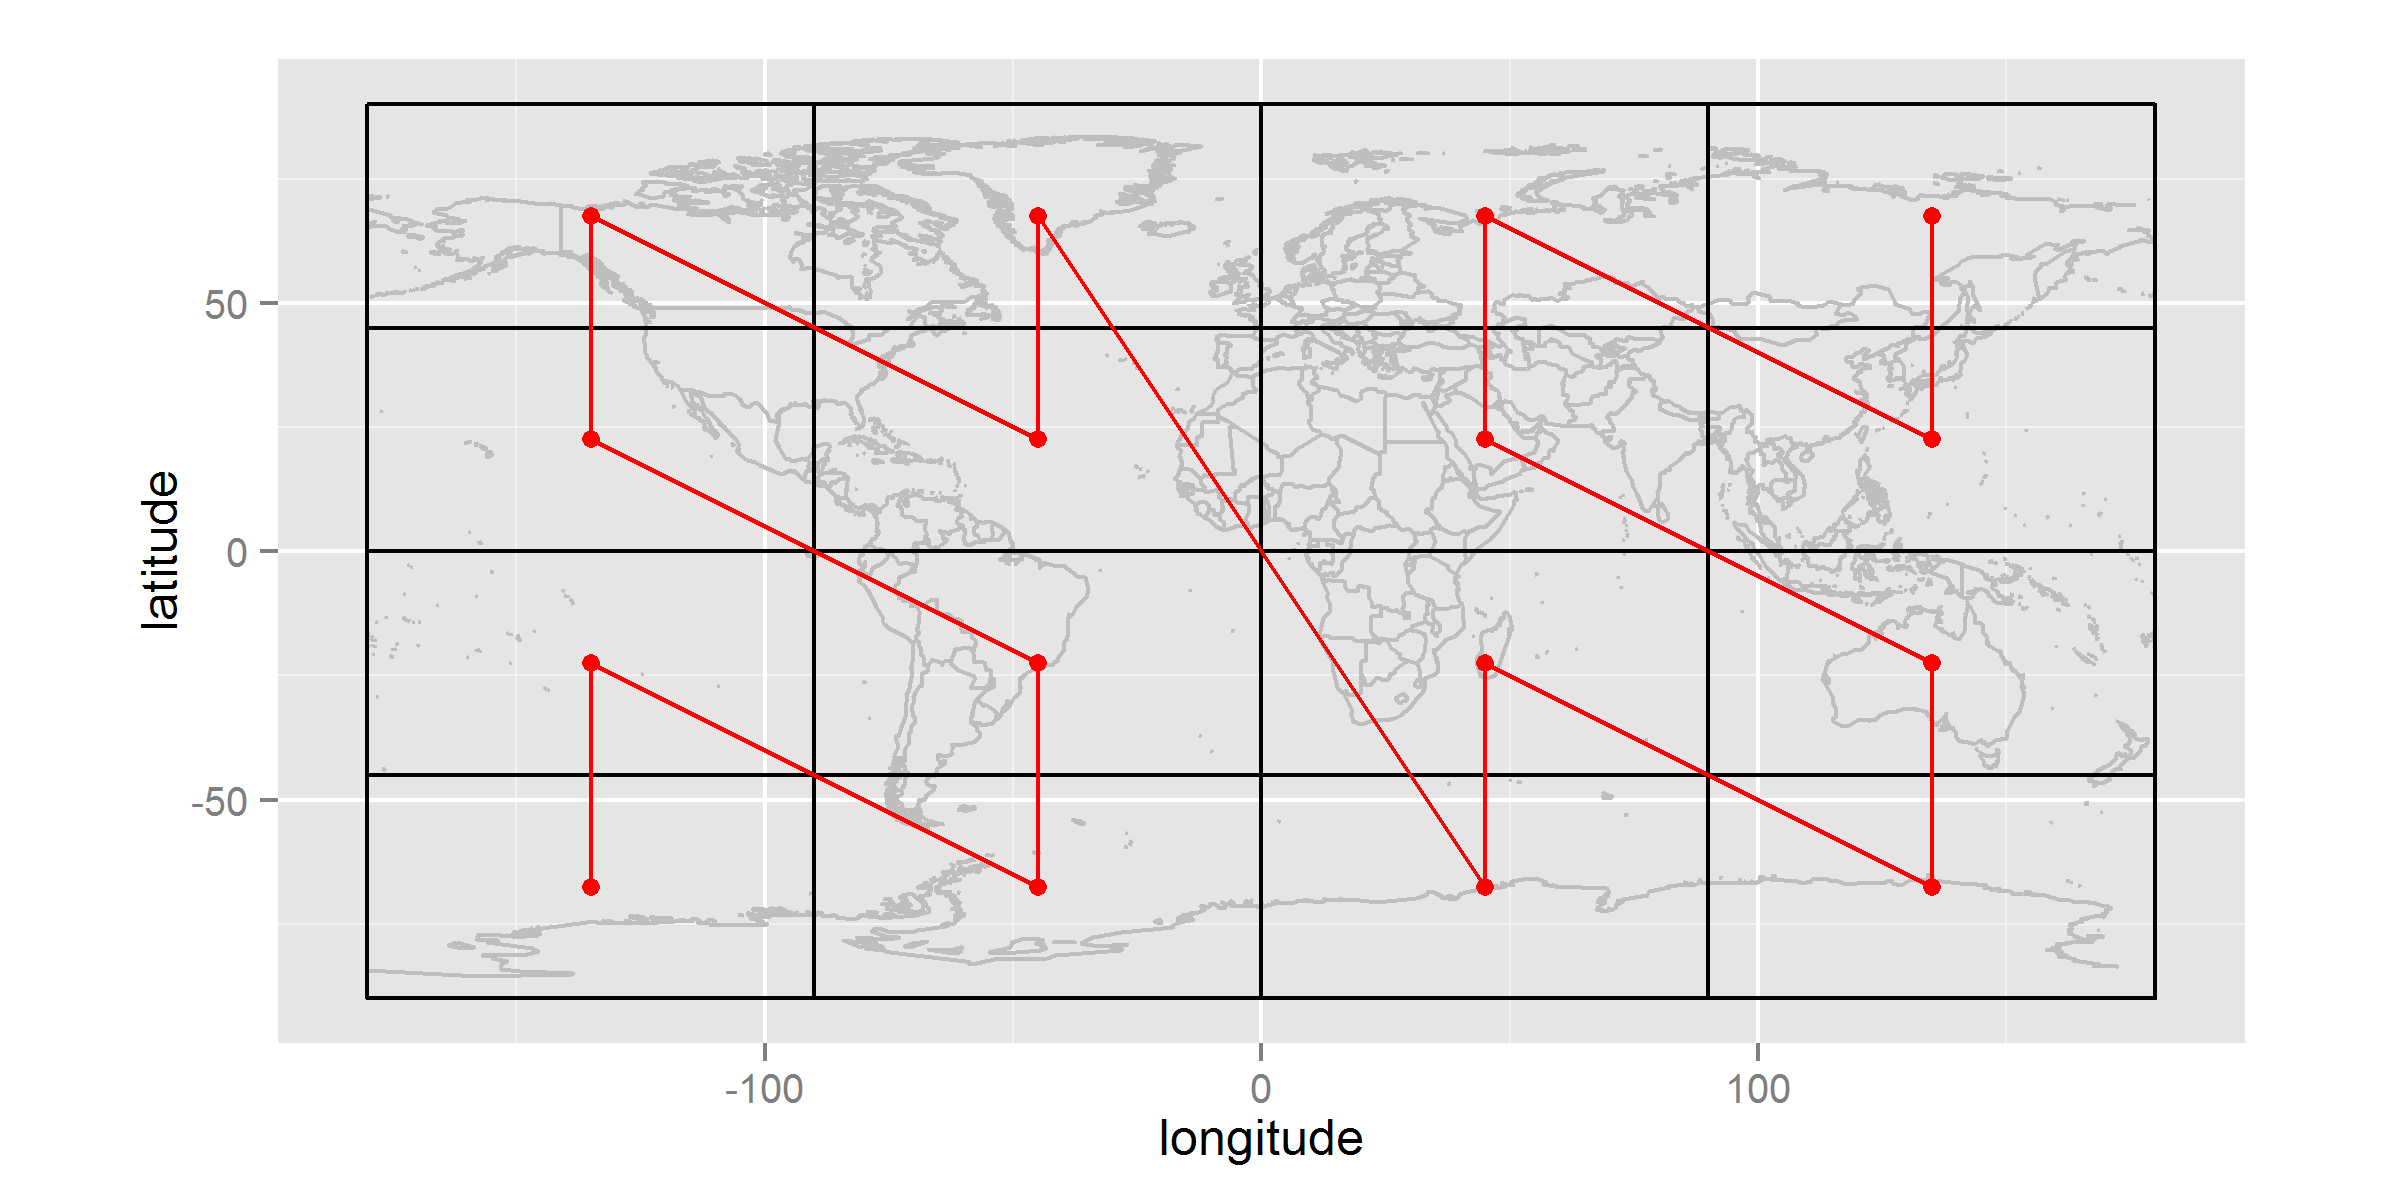
\includegraphics[width=\textwidth]{z_curve}
\caption{Z-order curve with precision 4 (\citet {spatiotemporal})}
\label{fig:zcurve}
\end{figure}

Figure \ref{fig:zcurve} shows all geohashes with precision 4, sorted and plotted with lines drawn between neighbouring elements. It is a mathematical object called z-order curve \cite{zcurve} and it appears at any chosen precision. It is also a good way to visualise how geohasing preserves locality.

\section{Key-value stores} \label{key-value}
Key-value stores are non relational databases.
As mentioned before geohashes provide a way to map two dimensional data into one dimension while preserving locality. It was also showed how to cover a rectangle with only few geohash ranges. This means that the system has to be able to retrieve all geohashes from a certain range. If all geohashes are stored in a sorted set, it is possible to find the first element from the range and iterate until the end of the range. As mentioned, rectangle coverage usually covers more area than requested, which means that when each element is returned from the set it has to be checked wether it really is within the rectangle.

This is where distributed key-value stores come to play. The criteria is that this data store is able to store keys in some sort of a sorted manner. One of the initial requests is that persistence is optional, and real time performance is more important. That's why a \emph{distributed in-memory database} is the best solution.

In few other relevant papers where they built spatial \cite{spatialindex} and spatio-temporal \cite{spatiotemporal} distributed indexes, they used HBase and Accumulo both based on Google's BigTable implementation. We didn't go with that choice because those are not in-memory databases.

We chose \emph{Redis} which is an in-memory key-value store with support for many different data types, and one of them is an ordered set called \emph{ZSET}. Originally Redis wasn't a distributed database, but in the past few years Redis Cluster was developed. Redis Cluster shards the data based on its key, but it can not shard within a single key which is needed because we would like to store all the geohashes inside a single key of type ZSET. This means that we will have to handle this part manually, by creating multiple ZSET keys and querying the appropriate ones.

ZSET orders elements by their score, which is a 64-bit floating point number that can store integer values without the loss of precision only if value is in range $[-2^{53}, 2^{53}]$. This score will be used to store geohash values with \emph{52 bit precision}. Those 52 bits are more than enough -- latitude resolution with 26 bits is $180^{\circ}/2^{26} \approx 2.6^{\circ}*10^{-6}$, or about 10 cm. Along with score, each element can store a string value called \emph{member}. It will be used to store a vehicle id.

Even though all point data is contained within each element of sorted set, some implementations will require an efficient way to lookup a vehicle location by its id. This is achieved using standard get and set methods to get or set a value on specified key. As previously said, Redis Cluster automatically shards data by its key, so this information doesn't have to be manually sharded as with ZSET.

\chapter {Algorithms} \label {algorithms}
In order to be able to answer a rectangle query it is necessary to have an algorithm that can find geohashes that cover an arbitrary rectangle completely. This is known as a \emph{rectangle coverage} problem. One goal is to use as few geohashes as possible and the other goal is to "over cover" the smallest possible area. If the second goal didn't exist, the solution would always be to use an empty geohash because it covers every rectangle. On the other side, if we wanted to perfectly cover the rectangle, it might happen that infinite number of geohashes are required.

To do this with respect to both goals we explain a simple algorithm in the section \ref{rect_cov}.
Section \ref{single_key} explains how to use the list of ranges that the algorithm produces to make a simple version of the system that stores all the points within a single set. Sections \ref{prefix} and \ref{vehicle_id} present two solutions on how to shard the data into multiple sorted sets to achieve scalability and better performance.

\section {Rectangle coverage} \label {rect_cov}
The first step of the algorithm is to compute the precision of the geohashes that will be used to cover the rectangle. To make the algorithm simpler, all the geohashes that cover the rectangle will be of the \emph{same} precision.
The idea is to find a central geohash -- one that covers the center point of the rectangle, and then find all eight neighbouring geohashes and return them with the central geohash. In the figure \ref{geohash_grid}, the central geohash is marked with the letter C, and the neighbouring geohashes are marked using letters for cardinal directions.

All that is left to do is to find the largest geohash precision that guarantees that the whole rectangle gets covered with those nine geohashes. To analyse the condition on one dimension, e.g. longitude, we will define $W$ as the length of the longitude side of the rectangle and $G$ as the length of the geohash longitude range at the current precision level. The condition that needs to hold at certain precision level is that $2*G \ge W$. If that condition holds, it means that the central geohash and it's left and right neighbour definitively cover the longitude range. Take a look at the figure \ref{geohash_condition} to better understand the condition, red line represents the query range and blue line represents the geohash ranges. Middle point $M$ will always be within the range of the central geohash (middle blue line). The edge case is when the left edges have the same value and $M$ is farthest to the left. In this case $G=W/2$ and if $W$ was any larger, the geohash ranges wouldn't cover the query, which gives inequality $G \ge W/2$.

The central geohash is constructed bit by bit, similarly to how geohash is encoded. At each step the condition needs to be checked, when it gets violated, the algorithm terminates and the last bit is removed. Take a look at the listing \ref{code:central} for the Python code that shows how the central geohash is calculated.

\label{code:central}
\begin{lstlisting}[language=Python, caption=Finding central geohash]
def find_central_geohash(x0, y0, x1, y1):
  def split_range(lo, hi, p):
    mid = (lo+hi)/2
    if p <= mid:
      return ('0', lo, mid)
    return ('1', mid, hi)

  x_min, x_max = -180, 180
  y_min, y_max = -90, 90
  x = (x0 + x1) / 2
  y = (y0 + y1) / 2
  central = ""
  for length in range(52):
    if length % 2 == 0:
      bit, x_min, x_max = split_range(x_min, x_max, x)
      g = x_max - x_min
      w = x1 - x0
    else:
      bit, y_min, y_max = split_range(y_min, y_max, y)
      g = y_max - y_min
      w = y1 - y0

    if 2*g >= w:
      central += bit
    else:
      break
  return central
\end{lstlisting}

\begin{figure}[h]
% trim = left, bottom, right, top
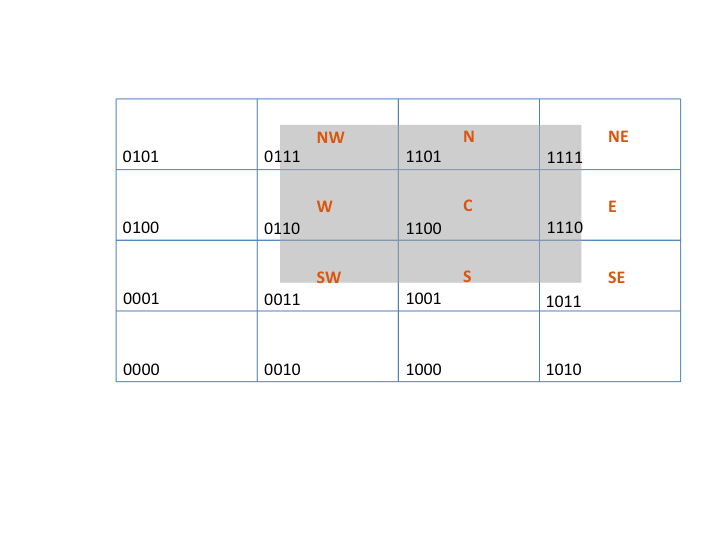
\includegraphics[width=\textwidth, trim=105 150 25 85, clip]{geohash_grid/Slide1}
\caption{Rectangle coverage with 4-bit geohashes}
\label{geohash_grid}
\end{figure}

\begin{figure}[h]
% trim = left, bottom, right, top
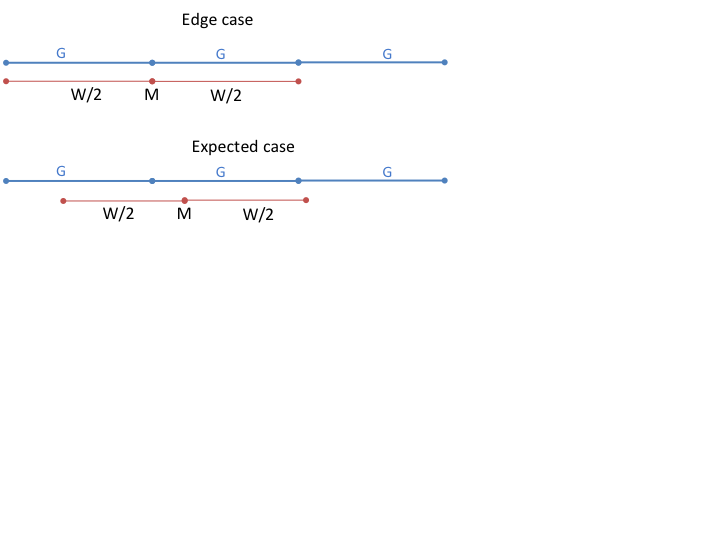
\includegraphics[width=\textwidth, trim=0 320 250 0, clip]{geohash_grid/Slide2}
\caption{Rectangle coverage condition}
\label{geohash_condition}
\end{figure}


This approach returns nine geohashes, but it might happen that not all of them even intersect the original rectangle, so those can be omitted. It turns out if the returned geohashes are sorted, then many of the neighbouring elements will differ only by one. This starts to make sense if you take a look at Figure \ref{fig:zcurve} where you can see how the consecutive geohashes are ordered on the map -- very often two consecutive geohashes are neighbours in one of the eight directions which is also the pattern of the returned geohashes. Instead of returning a list of geohashes, we can return a list of geohash ranges that cover the rectangle. In our example the returned geohashes are: 0011, 0110, 0111, 1001, 1011, 1100, 1101, 1110, 1111, or written in ranges form 0011--0011, 0110--0111, 1001--1001, 1011--1111.
Empirically, this resulting list of ranges usually has three or four elements which is much better than nine elements in the original list.

It is also important to understand how much area will the returned geohashes cover. The worst case in one dimension is when $G$ is maximised such that the condition doesn't hold at the next level. This is when $G' < W/2$, where $G'$ is geohash size at the next precision level, i.e. $G' = G/2$. When substituted and simplified we get $G < W$. This means that the worst case is when $G$ gets very close to $W$. Then, the covered length is $3W$ and over covered is $2W$. If this case is used in both dimensions, the covered area is $9W^2$ and the useful part is only $W^2$ which means 9 times more area was covered than the original rectangle size. Note, that this is not really the worst case when analysing the problem in two dimensions because one rectangle side can be 100 times larger than the other side. In this extremely asymmetrical case the algorithm will stop as soon as the geohashes become to small to cover the big side of the rectangle which produces geohashes with side length with the order of magnitude of the biggest side. This means that the covered area will be few hundred times bigger then the rectangle area. The only way to reduce the over covered area is to return more geohashes that approximate the rectangle more precisely.

\section {Single key solution} \label {single_key}
Before presenting distributed solutions, it is best to describe how to use geohashes and Redis on a single machine. In section \ref{key-value} we explained how to store 52-bit geohashes within a sorted set ZSET. A single ZSET instance is stored under a single key name that we will call K. It is not possible to shard within a single key, but exactly defining the algorithm that works on a single key is a good first step.

Updating a point is as simple as calculating its hash and performing an add function on the set. The exact Redis command is ZADD K geohash(lat, lon) vehicle\_id. It inserts a new point to the set if no point with the same vehicle id exists yet, otherwise it just updates its geohash and this is exactly the behaviour we need.

Doing rectangle queries requires consists of two steps:
\begin{itemize}
\item Use rectangle coverage to get the list of geohash ranges that cover the rectangle.
\item Make a query to Redis for each range $[A, B]$ using \texttt{ZRANGEBYSCORE K A' B' WITHSCORES}. It returns vehicle ids with their geohashes of all points with geohash in range $[A', B']$ (inclusive). Notice that we didn't use $A$ and $B$ to specify range because all of the stored geohashes are 52-bit numbers and $A$ and $B$ usually have much less bits. If they were used to query the data, usually no points would be returned. To obtain $A'$ and $B'$, $A$ and $B$ need to be filled up until 52 bits, $A$ with zeros and $B$ with ones. Range $[A',B']$ includes all 52-bit geohashes whose prefix is in range $[A,B]$.
\item Filter query results to eliminate all the points outside of the rectangle.
\end{itemize}

Most of the operations with sorted sets have a logarithmic complexity. Therefore update complexity is $O(log\ n)$ on a set with $n$ elements. Range query has complexity of $O(k + log\ n)$ where $k$ is number of elements returned by the query. Rectangle query consists of a constant number of range queries, usually three or four. This is why we can say that its complexity is $O(k + log\ n)$. Depending on the rectangle size, $k$ might be the one that prevails, or $n$. Ideal complexity would be without $log\ n$, but this is very close. Notice, that $k$ is the number of points before filtering the results. In practice $k$ is on average three times larger than the number of points in the actual rectangle.

\section {Prefix sharding} \label {prefix}
One way to distribute keys is to create more keys then the number of nodes and hope that approximately the same number of keys ends up on each node. Just as geohashing preserves locality, it is useful to try to do the same when designing the sharding scheme. This is achieved by sharding based on geohash prefix. When a point is added to the system, geohash is computed and it is inserted into one of the sorted sets based on its first $P$ bits. Each set is named based on the prefix it represents and all of the points inside that set share the same prefix. $P$ is an adjustable parameter that can be tuned based on the expected data set. Each prefix set is created lazily -- only when a point with such prefix is inserted.

When describing how to insert a point, we didn't mention how to do the update query. In most of the cases update query works without any modifications to the single key version. A problem arises when a vehicle location changes enough that it causes a change in the first $P$ bits. The new location will be inserted in a different prefix set, and the old location won't be deleted from the old set. If you recall from section \ref{key-value} that vehicle locations can be looked up by their id, then it is possible to partially resolve this problem by deleting a point from the prefix set that it used to belong to. This still won't resolve a problem when there are multiple updates for the same vehicle id and if both of the new locations belong to a different prefix set. The race condition is when both updates read the old location and delete it from its prefix set and then both of them insert the new location into two different prefix sets. Current implementation doesn't attempt to resolve any of these issues.

As already said, rectangle query boils down to answering what points are in a geohash range. It is possible that the queried geohash range spans through multiple prefix sets, so a range might be split in multiple ranges such that each of them contains only geohashes with the same prefix. For example, $P=3$ and queried range is $[\mathbf{101}01-\mathbf{111}00]$. It actually spans through three prefix sets $101$, $110$, $111$. Query range for each of those needs to be $[\mathbf{101}01-\mathbf{101}11]$, $[\mathbf{110}00-\mathbf{110}11]$ and $[\mathbf{111}00-\mathbf{111}00]$.

Choosing $P$ has a big impact on performance, not so much on updates as on rectangle queries. Larger $P$ creates smaller area that the prefix covers. If rectangle query has larger size than area covered by geohash prefix $P$, the range query will have to be split in multiple range queries. Let's define $G$ as the length of the geohash from the range query. Geohash of length $P$ covers $2^{-P}$ part of the total space, and $G$ covers $1/2^G$ part. One geohash from the range query contains $2^{-G}/2^{-P}$, or simplified $2^{P-G}$ geohashes that represent prefix sets. We always aim to have this number smaller than 1 to make the probability of splitting the range very small. On the other side we want to make $P$ big enough so the load gets distributed evenly. If rectangle queries are expected to be uniformly distributed all over the world then choosing $P$ to be six or seven is enough, but if we expect all queries to be in one city then $P$ has to be a lot larger. In our test cases $P$ is 22 because all the queries are within Beijing, if it was the whole Earth we would have to use a smaller number such as 7.

Obvious advantage with this approach is that the rectangle query is very fast, if $P$ is chosen appropriately and in most cases it doesn't make any more requests to Redis than the non-distributed variant.

Downside is that $P$ has to be chosen in advance. If it has to be changed later, all points need to be reinserted. A bit more subtle issue is that its performance is sensitive to spatial distribution of queries. When  $P$ is four, prefix sets divide the space as in figure \ref{geohash_grid}. Imagine that all rectangle queries suddenly start to hit small area within geohash 1011. This means that all queries would end up hitting a single sorted set and performance would downgrade as if there was no sharding, just as single key solution.

\section {Vehicle id sharding} \label {vehicle_id}
Another idea is to decide on the number of sorted sets $S$ and define a mapping between vehicle id and a set it belongs to. Each set stores a portion of data, but data is not sharded based on location, instead it is sharded based on vehicle id. This means that there is no spatial locality within a single set as was the case with prefix sharding. To get the best performance it is important for sets to be approximately the same size, which means that we must have a function that maps vehicle id to set id such that each set id gets approximately the same number of vehicle ids. This is why hash of vehicle id modulo $S$ is used for mapping. For convenience, the hash function used is the same one that Redis uses to map keys to slots when sharding keys between nodes.

Updating a point location is simple, hash the vehicle id to find the set it maps to and add it to the set. Rectangle queries are also simple to answer because we can use the single key solution on each of the sets. More precisely, rectangle coverage returns list of ranges and each of those ranges is used to query each of the $S$ sorted sets. Results are then merged, filtered and returned to the client. The downside is that each query needs to do the same operations with all of the $S$ sets which means $S$ times more queries to Redis than with a single key implementation. \emph{Total complexity} gives insight in the total load of the system, but \emph{complexity per node} is also useful because nodes work in parallel so we can say that it is the complexity as seen from clients perspective. Let $n$ be the total number of vehicle ids, and $k$ the total number of returned elements. Expected number of points in each set is $n/S$ and expected number of returned points per set is $k/S$. Complexity per each node is $O(k/S + log\ n/S)$. Total complexity is $O(k + S*log\ n/S)$ which gives $O(k + S*log\ n - S*log\ S)$ and $S*log\ S$ is a small constant that can be ignored to get a simpler complexity $O(k + S*log\ n)$. This is only a computing complexity, which isn't any worse than with single key solution, and per node complexity is even smaller, but we won't always see an improvement in throughput because there is also a lot of network overhead involved.

Usually, we can't tell which key will end up on which Redis node, so we initially used $S$ few times larger then the number of nodes to ensure approximately the same number of sets on each node. To lower the overhead we forced each set on its own node. To achieve this, it was necessary to rely on Redis internals. During Redis client initialisation, it gathers information about all Redis nodes. The main information gathered is to what node will each key hash map to. We use this information to decide in advance on the key name for each set before it is created. This way $S$ equals the number of nodes and performance is much better. The downside is if cluster is resharded, some sets  might end up on the same nodes, and the performance won't be so good.

Vehicle id sharding creates approximately equal load on all nodes, no matter what the spatial distribution of points or queries looks like. This might not seem like an important feature at first, but production systems often don't have the luxury to assume that some region on Earth won't suddenly become queried a lot more. Query response time and throughput should be better than a single key implementation, but the results won't be noticeable if queries are small because there is overhead to query each set and merge the results, and some sets might return zero results which only wastes resources without any performance gain.

\chapter {Design and implementation}
The latest Redis release 3.2.0. includes some geo features. In section \ref{redis_geo} we describe those features and explain how to compare them with solutions presented in this paper. Section \ref{setup} describes how the Redis cluster was setup and how it was used to measure performance of different implementations. Finally, section \ref{test} explains what kind of test data was used for measuring performance.

\section {Redis geo features} \label{redis_geo}
Redis geo features also have 52-bit geohashes in background, it is very similar to how a single key solution from section \ref{single_key} works. Two most important commands are GEOADD and GEORADIUS, to add a point and to query all points within certain radius. Points are also stored in a ZSET, within a single key. This means they share all the same drawbacks, mainly the lack of scalability.

Redis implementation only supports radius query, while and the implementations in this thesis support only rectangle queries. In order to compare performance between the two implementations we had to add radius querying capabilities to our implementation. To achieve this in the simplest possible way, it is best to reuse the existing rectangle query to answer the radius query. To do this we find the smallest possible rectangle that has the given circle inscribed in it and then filter out the points that are not within the circle. This is essentially the simplest algorithm for circle coverage, definitively not the most efficient one, but good enough to compare with the Redis implementation.

\section {Experimental setup} \label{setup}
Experimental setup has to components: \emph{Redis Cluster} and \emph{geo client}. Geo client contains all the logic about geo queries and issues as many requests to Redis as possible. It is a single threaded c++ application that uses asynchronous calls to Redis to achieve the best possible performance, even when compared to multithreaded synchronous client \citet{clientperf}.

Redis cluster uses a master slave model. All data is sharded by its key between masters, that is, each master contains a portion of the key space. This mapping is achieved by hashing the keys. Each master node forwards all commands to all of its slaves, and slaves eventually become consistent with its master. This is called \emph{replication} with number of slaves per master called \emph{replication count}. Replication is mainly used to provide high availability to the system, but this is not so important for this application so we chose only 1 replica per master node.
Redis is an in-memory database, but periodically flushes the data to disk to provide some level of persistency. When the flushing is in progress, Redis doesn't allow no updates to the database which can make performance measurements unpredictable. Also, on of the main reasons why Redis was chosen is because it is an in-memory database, and not its ability to efficiently persist data to disk. For these reasons, every persistency mechanism in Redis was disabled.

Redis Cluster has 6 machines in total, each machine equipped with quad-core processor. Each machine is running 2 masters and 2 slaves which totals to 12 masters and 12 slaves. 

We also used one machine in the same network to run geo clients on. Because of the single-threaded nature of geo clients, we were able to use multiple number of them on the same machine and still increase the load on the Redis cluster.

\section {Test data} \label{test}
The basis for the dataset used is T-Drive \citet{tdrive1, tdrive2} dataset. It is was recorded by 10000 taxi drivers in Beijing from Feb. 2 to Feb. 8, 2008. There is about 17 million points, but we used only 5 million for testing. Each datapoint consists of taxi id, timestamp, longitude and latitude. There is not enough taxis so we decided to ignore taxi id, and generate a new id to use as vehicle id for each data point. Timestamp is also irrelevant because we are not trying to make a trajectory of taxi movement or anything similar, just insert points without any temporal information. These data points are directly used in update queries.

Now, we need to figure out interesting rectangle and radius queries that can reflect the difference between different implementations, mainly prefix and vehicle id sharding. Each implementation might behave different for queries with different rectangle areas -- small or big. Prefix sharding should not scale well when there is one hot region, which is something that can be easily tested by creating queries that hit one area more than others. Generating rectangles whose centre points are generated by normal distribution is a perfect choice for this. Of course, there is also a data set with rectangles whose centres were generated by uniform distribution. All of the generated rectangles are within the area where T-Drive data points are. To sum up, there are four rectangle data sets: small uniform, big uniform, small normal and big normal.

Rectangle queries are created to show the differences between the three implementations described in chapter \ref{algorithms}. On the other hand, radius query was created because Redis geo features only support that type of query and we would like to compare solutions presented here with the native implementation. This is why there is no need to generate data sets with uniform and normal distribution, so we generated circle centres using uniform and radius using normal distribution. There are still small and big data sets to see how the implementations respond.

\chapter {Results}
All queries originate from one machine, possible from multiple clients that try to maximise the utilisation of one client machine by issuing as many queries as possible. Sometimes the bottleneck is the machine itself, and sometimes a single machine within a Redis cluster. In section \ref{rectangle_results} we present and explain the performance of rectangle queries under different implementations and in section \ref{radius_results} we explain how the radius queries compare with the native Redis implementation. The main metric measured is number of queries per second, interchangeably used with requests per second.

\section {Updates}
All update methods have a throughput between 120000-150000 requests per second. This is to be expected because every update method is essentially the same, geohash is computed and point is added to an appropriate sorted set. The only case were there might be a significant difference is if we tried to fix a problem with the prefix sharding's updating inconsistencies, but even that can be implemented almost as efficiently as the other methods.

\section {Rectangle queries} \label {rectangle_results}
The first tests ran were on uniform data sets. Small dataset had to retrieve 15 points on average while big data set had 3048 points on average. Out of the points retrieved approximately the third of them are actually within the queried rectangle, but we don't report it because the total points returned by Redis has more significance on performance. 

The most noticeable is a 100 times drop in performance seen between figures \ref{small_uniform} and \ref{big_uniform}, but it is not unexpected when the number of points returned is taken into account, which is also a 100 times difference. It makes sense because sorted set range search complexity rises linearly with the number of returned points.

\begin{figure}[h]
\minipage{0.49\textwidth}
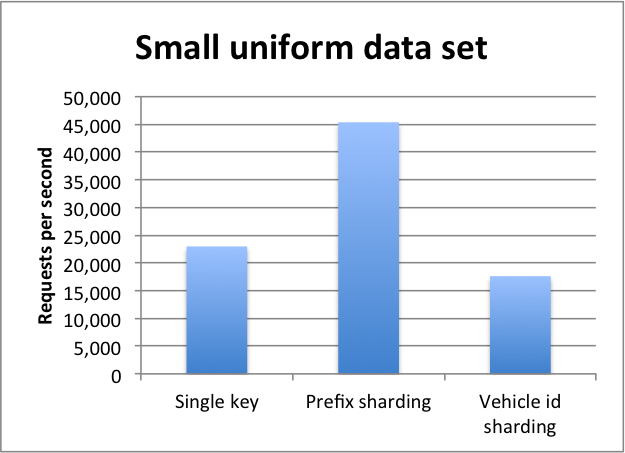
\includegraphics[width=\textwidth]{rectangle_small_uniform}
\caption{Rectangle query -- average points 15}
\label{small_uniform}
\endminipage\hfill
\minipage{0.49\textwidth}
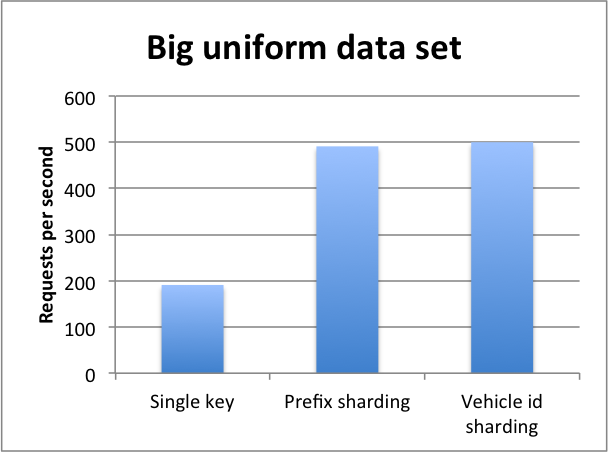
\includegraphics[width=\textwidth]{rectangle_big_uniform}
\caption{Rectangle query -- average points 3048}
\label{big_uniform}
\endminipage\hfill
\end{figure}

If we focus only on the small data set, then we see that the Prefix sharding algorithm was very successful, it managed to achieve two times better performance than others, mostly because it managed to spread the load among all of the Redis instances, while the single key implementation just utilised one node completely. As predicted, vehicle id sharding doesn't show improvements on small query sizes because overhead of contacting all of the nodes is too high compared with the gain of processing a request parallely. Big rectangle queries confirm that this is the case because the query rate evens out with prefix sharding.

\begin{figure}[h]
\minipage{0.49\textwidth}
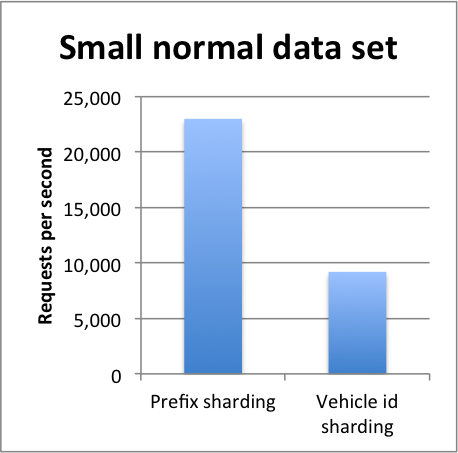
\includegraphics[width=\textwidth]{rectangle_small_normal}
\caption{Rectangle query -- average points 50}
\label{small_normal}
\endminipage\hfill
\minipage{0.49\textwidth}
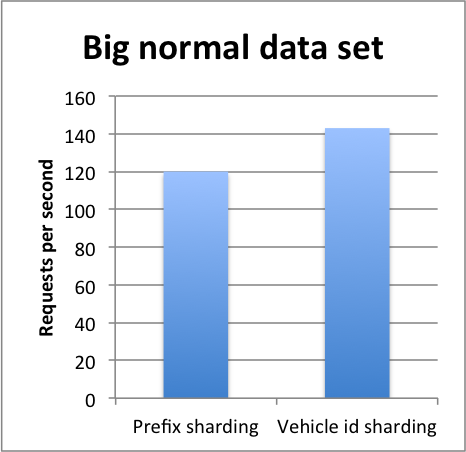
\includegraphics[width=\textwidth]{rectangle_big_normal}
\caption{Rectangle query -- average points 9711}
\label{big_normal}
\endminipage\hfill
\end{figure}

Figures \ref{small_normal} and \ref{big_normal} are ran on the data set generated by normal distribution. The goal is to try to find a case when vehicle id sharding outperforms prefix sharding. On the small data set vehicle id sharding is still much slower than prefix sharding, but on the big data set it outperforms prefix sharding by a small margin. The difference might get even bigger if more client machines are used to run the queries to make Redis even bigger bottleneck, but it is just a hypothesis.

\section {Radius queries} \label{radius_results}
Radius queries compare all three implementations with the Redis GEORADIUS command. It's implementation is most similar with the single key algorithm because both work within a single key on one node. Figure \ref{small_radius} shows that the Redis implementation has about 50\% bigger throughput than our single key version. The two main reasons for the performance gap are:
\begin{itemize}
\item Both implementations have to retrieve 3-4 times more data points than necessary to answer the query, but the implementation within Redis is able to filter them directly on the Redis node, thus avoiding the unnecessary network transfer.
\item To answer the query, circle has to be covered with a few geohash ranges which are then passed to Redis. When a client implements circle coverage the ranges have to be sent to Redis over the network which again causes additional overhead.
\item Single key implementation is designed to work with rectangle queries, with radius queries built on top of it by making a rectangle around the circle. This makes our implementation cover approximately 27\% larger area to begin with and can expect the number of points retrieved to be also that much higher.
\end{itemize}
Even with those limitations, prefix sharding and vehicle id sharding are able to outperform it. Prefix sharding is the clear winner on the small data set, and it wins by a small margin one the big data set.

\begin{figure}[h]
\minipage{0.49\textwidth}
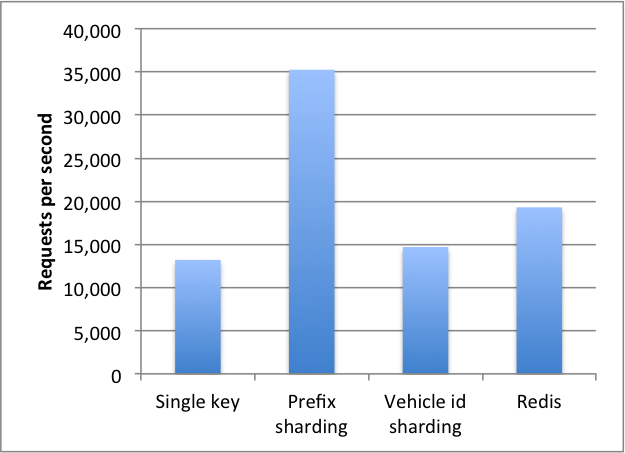
\includegraphics[width=\textwidth]{radius_small}
\caption{Radius query -- average points 10}
\label{small_radius}
\endminipage\hfill
\minipage{0.49\textwidth}
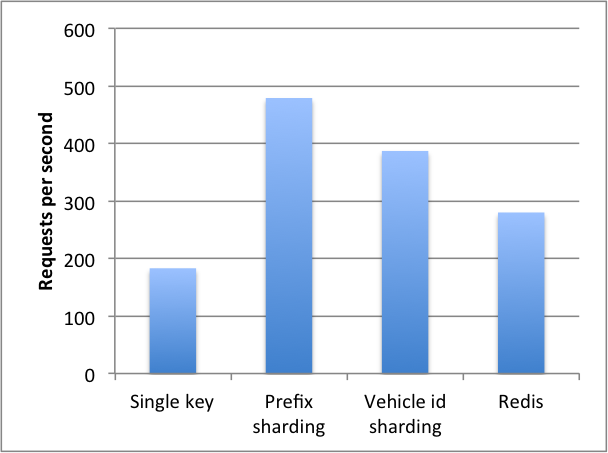
\includegraphics[width=\textwidth]{radius_big}
\caption{Radius query -- average points 1000}
\label{big_radius}
\endminipage\hfill
\end{figure}


\chapter{Conclusion}
We have described and implemented few ideas to build realtime system for tracking vehicle locations. In the hearth of the problem is the need for scalability beyond a single machine. Traditional solutions offer efficient and well established implementations but do not scale well. Ideas in this thesis are all based on translating the two dimensional data space to one dimension using geohash. This causes a completely different approach when designing algorithms so we focused only on minimal set of geo queries. Updating point locations and searching for points within a rectangle is the minimal set of queries. We used Redis as an efficient distributed in-memory key-value store, which is designed to shard the keys over a number of master nodes. The simplest solution to store all the points within a single key is described in section \ref{single_key}. However, this prevents scalability, so we found two ways to shard the data manually.

\begin{itemize}
\item Prefix sharding splits the data into multiple prefix sets. Each prefix set contains points with the same prefix of length $n$ where $n$ is parameter that has to be chosen in advance.

\item Vehicle id sharding shards the data based on the vehicle id which means that each node contains one sorted set, and updates for the same vehicle always end up on the same node.
\end{itemize}

Running performance tests revealed interesting use cases of each implementation. Prefix sharding performs much better than vehicle id sharding when queried rectangles contain small number of points. The two implementations even out when number of points inside queried rectangles is much higher. When performing those tests it was evident that the load is much more evened out when using vehicle id sharding, especially when the query data set was designed to hit one area much more often than others. The only test were vehicle id sharding was better than prefix sharding is on the big normal dataset but the margin wasn't big enough for it to be a convincing argument. To conclude, prefix sharding is definitively better if rectangle positions are uniformly distributed without the possibility of suddenly one region becoming very hot and therefore limiting the system throughput to only a single Redis node.

We also implemented the radius query on top of the rectangle query to be able to compare with the lastest Redis geo features. Our single key implementation had about 50\% lower throughput which is to be expected because these queries weren't built directly into Redis but on top of it.

\section {Future work}
There are several different paths for further investigation.
\begin{itemize}
\item Test the hypothesis that having more clients on more machines could in total have better request rate than the prefix sharding.

\item There is still a lot more possible queries that traditional R-trees can handle, one of the most popular is finding the K nearest neighbours (knn) from a given location. One idea for such implementation is to search in concentric circles with exponentially increasing radius until at least K points is returned from the system.

\item This thesis hasn't investigated how would creating a higher number of replicas in the cluster effect the performance. Those replicas could be used as readonly nodes to further increase the performance of the search queries, with the downside of having more stale data.

\item Improve Redis by sharding big keys that are otherwise stuck on only one machine. Starting point for sorted sets could be prefix sharding or vehicle id sharding.

\item Investigate if there are more appropriate storage solutions than Redis.
\end{itemize}


\bibliography{literatura}
\bibliographystyle{fer}

















% ----------------------------------Summary------------------------------------------------------
\begin{sazetak}
Sažetak na hrvatskom jeziku.

\kljucnerijeci{Ključne riječi, odvojene zarezima.}
\end{sazetak}

% TODO: Navedite naslov na engleskom jeziku.
\engtitle{System for tracking vehicle locations in real time}
\begin{abstract}
This thesis discusses design and implementation of the backend part of the distributed system for tracking vehicle locations in real time. Data sharding is necessary to distribute the system, which is achieved using geohashing. Redis Cluster is used as a distributed in-memory storage solution, on top of which we developed prefix and vehicle id sharding schemes. To correctly answer rectangle queries, rectangle coverage algorithm was developed, based on the ideas seen in few other codebases. We compare the two sharding schemes, single key solution and the recently developed geo queries in Redis. The latter two are non distributed versions and benchmarks show that distributed versions outperform them easily, but between prefix and vehicle id sharding there is no clear winner because on some test cases one is better and on some the other.

\keywords{Redis, Distributed, Geohash, Spatial index, Real-time}
\end{abstract}

\end{document}
